\documentclass[fontsize=12pt,paper=a4,twoside]{scrartcl}
\usepackage{longtable} 
\usepackage{graphicx}
% SWP-Präambel
% C 2003-2017 Sebastian Offermann, Rainer Koschke, Karsten Hölscher
% In Zeilen 40 und 41 sind jeweils die aktuellen Daten einzutragen

\usepackage[utf8]{inputenc}     % Kodierung der Tex-Datei
\usepackage[T1]{fontenc}        % Korrekte Ausgabe von Sonderzeichen (Umlaute)
\usepackage[ngerman]{babel}     % Deutsche Einstellungen [ab \begin{document}]

\usepackage{bibgerm}            % Bibliographie
\usepackage{fancyhdr}           % obere Seitenränder gestalten
\usepackage{float}              % Floats Objekte mit [H] festsetzen
\usepackage{graphicx}           % Graphiken als jpg, png etc. einbinden
\usepackage{moreverb}           % zusätzliche verbatim-Umgebungen
\usepackage{pdflscape}          % PDF-Support für landscape
\usepackage[final]{pdfpages}    % Externe PDFs einbinden
\usepackage{stmaryrd}           % zusätzliche Symbole
\usepackage{supertabular}       % Tabellen über Seitenränder hinaus
\usepackage{tabularx}           % Tabellen mit vorgegebener Breite
\usepackage{url}                % setzt URLs schön mit \url{http://bla.laber.com/~mypage}

%%% Die Reihenfolge der folgenden Pakete muss beibehalten werden:
%%% varioref, hyperref, cleveref, bookmark
% Verweise innerhalb des Dokuments schick mit " ... auf Seite ... "
% automatisch versehen. Dazu \vref{labelname} benutzen
\usepackage[ngerman]{varioref}  % [vor hyperref für korrekte Verweise]
\usepackage[colorlinks=true, pdfstartview=FitV, linkcolor=blue,
            citecolor=blue, urlcolor=blue, hyperfigures=true,
            pdftex=true]{hyperref} % [vor bookmark wegen der Optionen]
\usepackage[ngerman]{cleveref}
\usepackage{bookmark}

\hyphenation{Arbeits-paket}     % Trennungsregeln

%%% Definitionen
\newcommand{\grad}{\ensuremath{^{\circ}} }
\renewcommand{\strut}{\vrule width 0pt height5mm depth2mm}
\newcommand{\gq}[1]{\glqq{}#1\grqq{}}

%%% Semesterkonstanten
\newboolean{langversion} %Deklaration
\setboolean{langversion}{true} %Zuweisung ist 'false' für Blockkurs
\newcommand{\jahr}[1]{2020} %2017/2018

% erstes Argument: SWP-2, zweites SWP-1
\newcommand{\highlight}[1]{\textcolor{blue}{\textbf{#1}}}
\newcommand{\variante}[2]{\ifthenelse{\boolean{langversion}}{#1}{#2}}
\newcommand{\nurlangversion}[0]%
    {\variante{\highlight{}}%Muss in SWP-2 ausgefüllt werden}}%
              {\highlight{Entfällt in SWP-1}}}
\newcommand{\swp}[0]{Software-Projekt \variante{2}{1}}
\newcommand{\semester}[0]{SoSe \jahr}

%%% Formatierungsanpassungen
% Damit Latex nicht zu lange Zeilen produziert:
\sloppy
%Uneinheitlicher unterer Seitenrand:
%\raggedbottom

% Kein Erstzeileneinzug beim Absatzanfang
% Sieht aber nur gut aus, wenn man zwischen Absätzen viel Platz einbaut
\setlength{\parindent}{0ex}

% Abstand zwischen zwei Absätzen
\setlength{\parskip}{1ex}

% Seitenränder für Korrekturen verändern
\addtolength{\evensidemargin}{-1cm}
\addtolength{\oddsidemargin}{1cm}

\bibliographystyle{gerapali}

% 1. Parameter: Euer/Eure TutorIn, z. B. {Kim Harrison}
% 2. Parameter: Abgabedatum, z. B. {05. April 2063}
% 3. Parameter: Versionsnummer, z. B. {1.1}
% 4.-9. Parameter: jeweils Name und (Uni-)Email-Adresse jedes 
%                 Gruppenmitglieds; mit einem & getrennt, z. B.
% {Robin Cowl & roco@tzi.de}
% Besteht die Gruppe aus weniger als 6 Personen, so werden die 
% übrigen Parameter leer gelassen: {}
\newcommand \swpdocument[9] {
% Lustige Header auf den Seiten
  \pagestyle{fancy}
  \setlength{\headheight}{70.55003pt}
  \fancyhead{}
  \fancyhead[LO,RE]{\swp{}\\%
                    \semester{}\\%
                    \documentTitle}
  \fancyhead[LE,RO]{Seite \thepage\\%
                    \slshape \leftmark\\%
                    \slshape \rightmark}

% Lustige Header nur auf dieser Seite (Titelseite)
  \thispagestyle{fancy}
  \fancyhead[LO,RE]{ }
  \fancyhead[LE,RO]{Universität Bremen\\%
                    FB 3 -- Informatik\\%
                    Dr. Karsten Hölscher\\%
                    TutorIn: #1}
  \fancyfoot[C]{}

% Start Titelseite
  \vspace{3cm}
  \begin{minipage}[H]{\textwidth}
    \begin{center}
      \bfseries \Large \swp{} -- \semester{}\\
      \smallskip
      \small VAK 03-BA-901.02\\
      \vspace{3cm}
    \end{center}
  \end{minipage}
  \begin{minipage}[H]{\textwidth}
    \begin{center}
      \vspace{1cm}
      \bfseries \Large \documentTitle\\
      \vfill
    \end{center}
  \end{minipage}
  \vfill
  \begin{minipage}[H]{\textwidth}
    \begin{center}
      \sffamily
      \begin{tabular}{lr}
        #4 \\
        #5 \\
        #6 \\
        #7 \\
        #8 \\
        #9 \\
      \end{tabular}
      \\[22mm]
      \itshape Abgabe: #2 --- Version #3 \\ ~
    \end{center}
  \end{minipage}
% Ende Titelseite

% Start Inhaltsverzeichnis
\newpage
  \thispagestyle{fancy}
  \fancyhead{}
  \fancyhead[LO,RE]{\swp{}\\%
                    \semester{}\\%
                    \documentTitle}
  \fancyhead[LE,RO]{Seite \thepage\\%
                    \slshape \leftmark\\~}
  \fancyfoot{}
  \renewcommand{\headrulewidth}{0.4pt}
  \tableofcontents
% Ende Inhaltsverzeichnis

% Header für alle weiteren Seiten
\newpage
  \fancyhead[LE,RO]{Seite \thepage\\%
                    \slshape \leftmark\\%
                    \slshape \rightmark}

}



%
% Und jetzt geht das Dokument los....
%
\begin{document}
\newcommand\documentTitle{Benutzerhandbuch}
 %\begin{minipage}[b]{\textwidth}
 \vspace{1mm}
 \begin{figure}[!b]
  \centering
  
\includegraphics[width=0.5\textwidth]{pics/SpaceStudioLogo.png}\\
\end{figure}

\swpdocument{Dr. Karsten Hölscher}{02. August 2020}{1.1}%
            {Clara Maria Odinius & odinius@uni-bremen.de}%
            {Habib Mergan & habib1@uni-bremen.de}%
            {Kevin Santiago Rey Rodriguez & kev\_rey@uni-bremen.de}%
            {Liam Hurwitz & hurwitz@uni-bremen.de}%
            {Mehmet Ali Baykara & baykara@uni-bremen.de}%
            {Miguel Alejandro Caceres Pedraza & mcaceres@uni-bremen.de}%

%%%%%%%%%%%%%%%%%%%%%%%%%%%%%%%%%%%%%%%%%%%%%%%%%%%%%%%%%%%%%%%%%%%%%%%%



%%%%%%%%%%%%%%%%%%%%%%%%%%%%%%%%%%%%%%%%%%%%%%%%%%%%%%%%%%%%%%%%%%%%%%%%
\section{Einführung}

Willkommen beim Spacestudio Game!\\
Dieses Benutzerhandbuch beschreibt, wie die Software bzw. das Spiel gespielt wird und dient somit als Anleitung für das Programm.
Lesen Sie sich dieses Handbuch aufmerksam durch bevor Sie die Anwendung starten, um alle Funktionalitäten des Spiels kennen zu lernen und zu verstehen.

Dieses Spiel ist nach dem Vorbild des bekannten Spiels Faster Than Light entwickelt worden, daher werden Sie viele Parallelen zwischen diesen beiden Spielen feststellen können.

%%%%%%%%%%%%%%%%%%%%%%%%%%%%%%%%%%%%%%%%%%%%%%%%%%%%%%%%%%%%%%%%%%%%%%%%
\subsection{Zweck}

Dieses Benutzerhandbuch ist im Rahmen von ReSWP 2 SoSe2020  der Gruppe SpaceStudio geschrieben.
Der Zweck dieses Handbuches besteht darin, eine Anleitung zu dem entwickleten Spiel bereit zu stellen, damit sowohl das Spiel selbst, als auch unsere Gedanken und Ideen bezüglich der vielen einzelnen Elemente nachvollzogen werden können.

%%%%%%%%%%%%%%%%%%%%%%%%%%%%%%%%%%%%%%%%%%%%%%%%%%%%%%%%%%%%%%%%%%%%%%%%

\section{Installation}
In diesem Abschnitt wird beschieben, wie das Programm installiert wird und entsprechende Systemvoraussetzungen aufgelistet.

\subsection{Systemvoraussetzungen}
1. Java 11 Oracle oder höher \\
2. Windows 10, macOS, Linux \\
3. Gradle 5.2 oder höher \\
4. 1920X1080 Auflösung (optimal)
 

\subsection{Installationsschritte}
Folgende  Schritte werden für die Installation benötigt. \\
 Nach dem Sie alle benötigten tools, die in Systemvoraussetzungen aufgelistet wurden, installiert haben \\
Linux installation
1. Starten Sie den Server mit folgendem Command: ./gradlew bootRun\\
2- Starten Sie den Client mit folgendem Command:  ./gradlew :Client:desktop:run \\

Windows Installation \\

1. Starten Sie den Server mit folgendem Command: gradlew.bat bootRun\\
2- Starten Sie den Client mit folgendem Command:  gradlew.bat :Client:desktop:run \\


\subsection{Troubleshooting}
** Known Issues\\
Failure in Server initialisation. If the Server does not let you create users after start up. You need to restart the Server.\\
If you experience memory leaks, while starting runs "pkill java" on unix system to resolve these Issues.\\
The Bugs are in Spring Boot and in Java\\


%%%%%%%%%%%%%%%%%%%%%%%%%%%%%%%%%%%%%%%%%%%%%%%%%%%%%%%%%%%%%%%%%%%%%%%%

\section{Start}

Startet der Client, dann zeigt sich sich der Registrierungs und Login Screen.
Registrieren Sie sich über die Eingabefelder auf der rechten Seite. Dazu wählen Sie einen Benutzernamen und Passwort, welches zwei Mal wiederholt eingegeben werden muss, um fehlerhafte Eingaben zu vermeiden.
War die Registrierung erfolgreich, bekommen Sie die Rückmeldung Successfully created, anderen falls erscheint Password does not match oder sofern der Benutzname schon vergeben wurde Name already
registered, try another one.\\
Nach erfolgreicher Registrierung geben Sie ihre Benutzernamen und Passwort in die linken Eingabefelder ein, ist auch der Login erfolgreich erscheint die Rückmeldung login... .\\

Hinweis: Gib es Probleme mit der Registrierung, empfehlen wir den Server erneut zu starten.

\subsection{Anmeldung}
\begin{figure}[htp]
\centering
	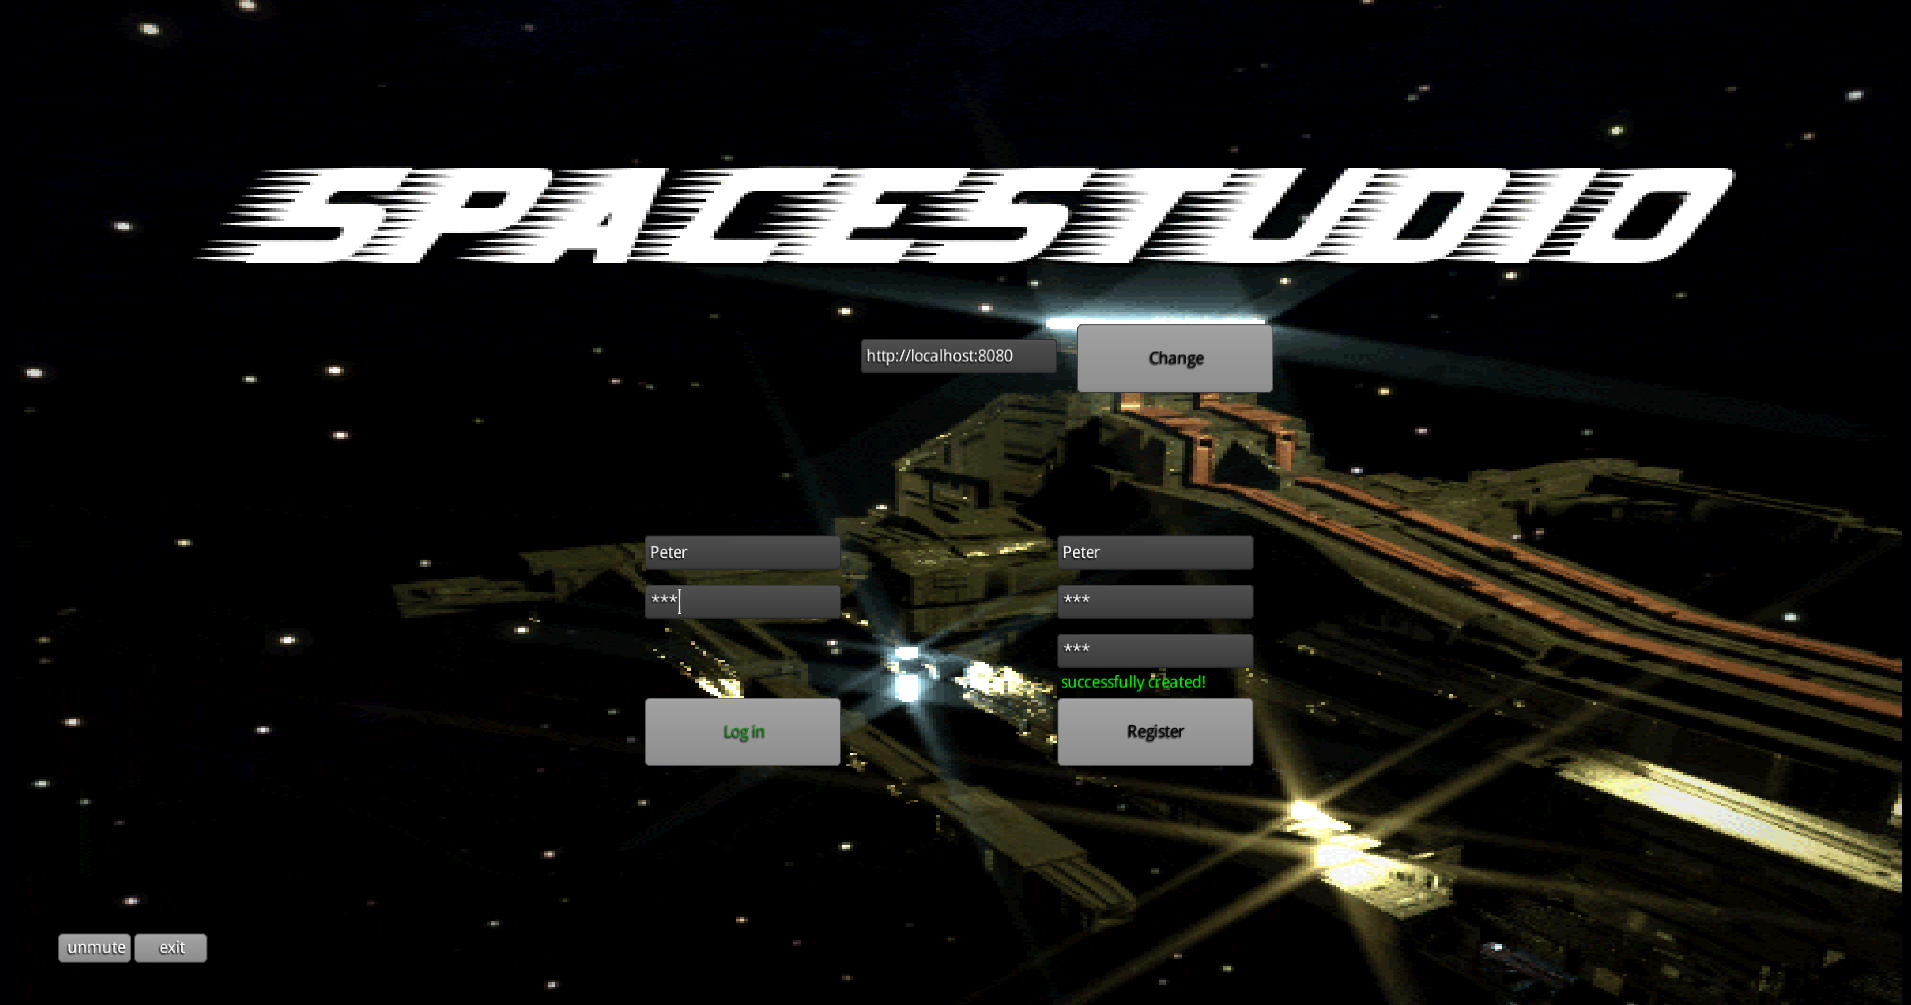
\includegraphics[width=1.00\linewidth]{pics/StartScreen01.png}
	\caption{Anmeldung: Registrierung und Login}
	\label{fig1}
\end{figure}

Der Start Screen erzeugt ein Profil, mit welchem sich der Benutzer jeder Zeit wieder einloggen kann, um auf die gespeicherten Spieldaten zurückgreifen zu können. \\
Darüber hinaus besteht die Möglichkeit, eine Netwerkadresse einzugeben, falls zu einem Späteren Zeitpunkt der Multiplayer-Modus gewählt wird, dazu mehr im Kapitel Multiplayer-Modus.\\
In der unteren linken Ecke des Fensters befinden sich die zwei Button mute und exit. Über den Mute-Button lässt sich die Hintergrundmusik an- und ausschalten. 
Über den Exit-Button kann das Spiel ohne weiteres beendet werden.

\newpage

%%%%%%%%%%%%%%%%%%%%%%%%%%%%%%%%%%%%%%%%%%%%%%%%%%%%%%%%%%%%%%%%%%%%%%%%
\subsection{Menu}

Nach dem Registrierungs und Login Screen folgt das Menü:\\
Zu sehen sind die drei Button New Game, Options und Exit. Sofern vorher schon ein Spiel begonnen wurde, erscheint auch der Button Continue.\\

\begin{figure}[htp]
	\centering
	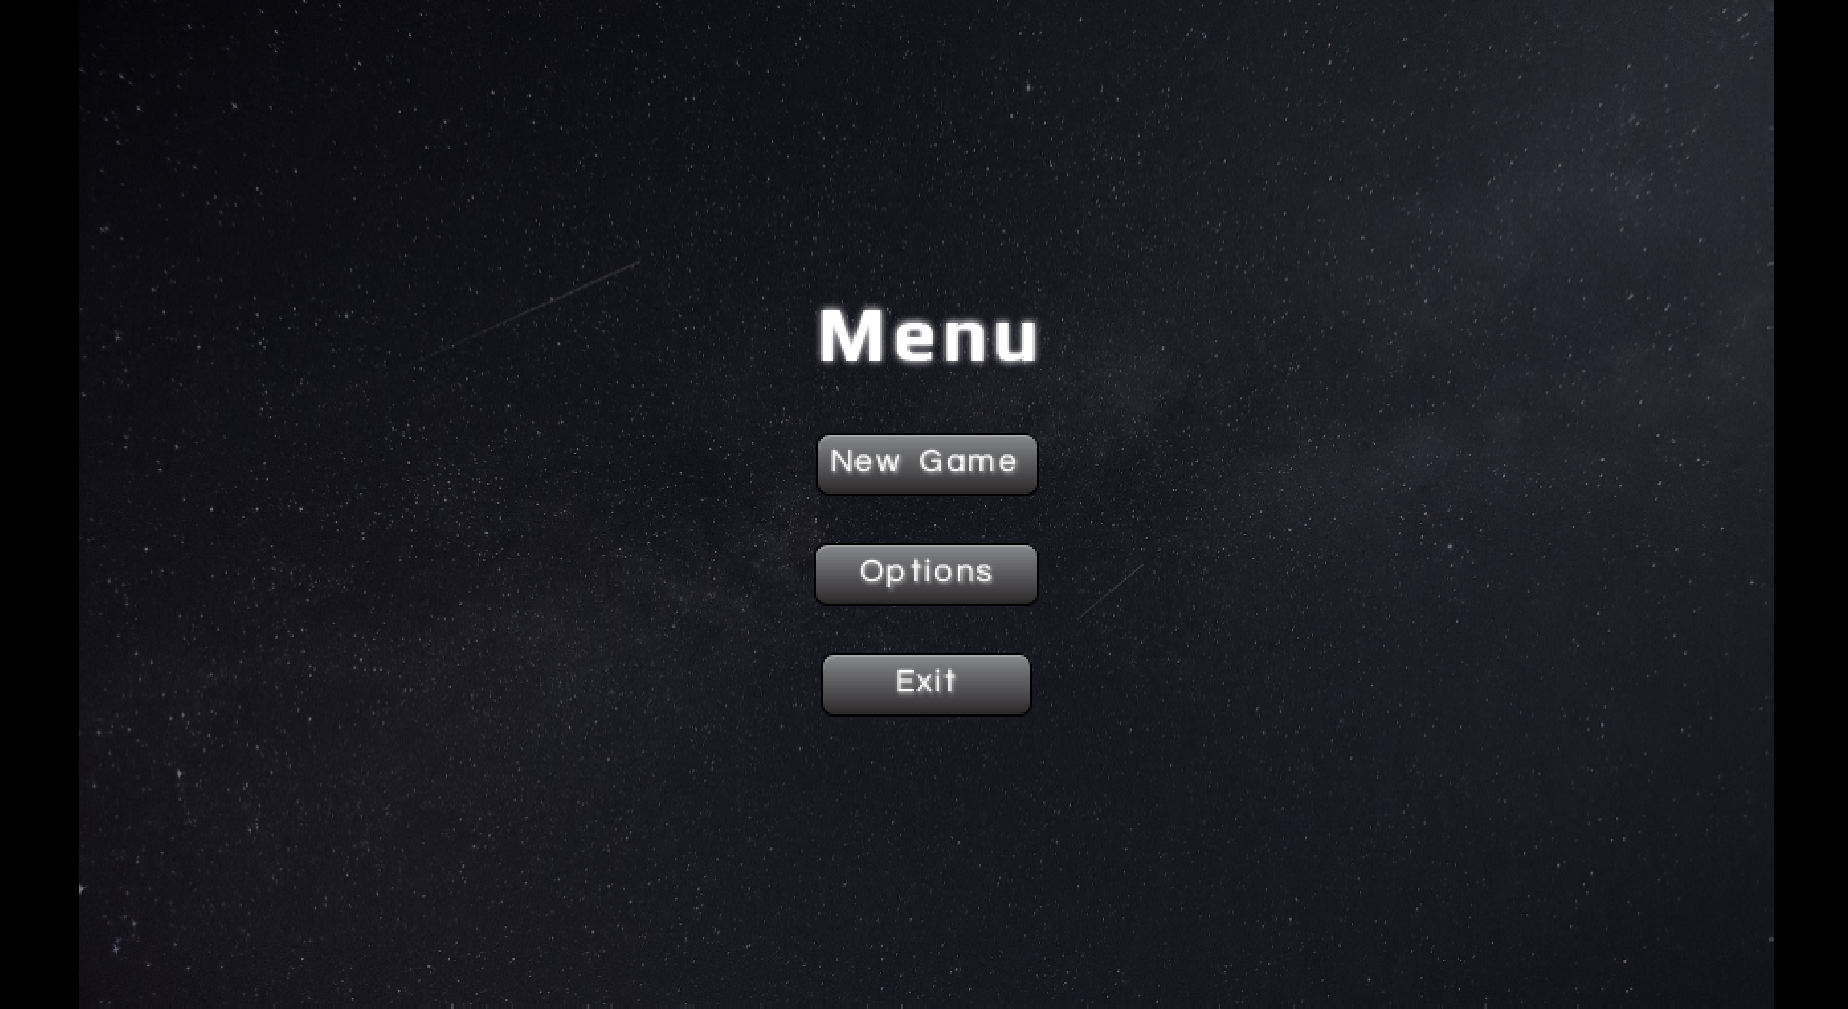
\includegraphics[width=1.00\linewidth]{pics/menuscreen.png}
	\caption{Menu}
	\label{fig1}

\end{figure}

Über New Game kann ein neues Spiel begonnen werden. \\
Continue ermöglicht es, ein zuvor begonnenes Spiel weiter zu Spielen, da jeder Spielstand gespeichert werden kann.\\
Options ist derzeit nicht verfügbar und kann für persönliche Anpassungen implementiert werden. \\
Exit beendet das Programm umgehend, ohne zur Startseite zurück zu gelangen.\\

\newpage
%%%%%%%%%%%%%%%%%%%%%%%%%%%%%%%%%%%%%%%%%%%%%%%%%%%%%%%%%%%%%%%%%%%%%%%%
\subsection{New Game}

Sofern im Menu Screen new Game ausgewählt wurde, folgt der New Game Screen.\\
Hier ergeben sich die Möglichkeiten ein Single Player Spiel oder ein Multiplayerspiel zu starten, oder aber zurück zum Menü zu gelangen.\\

\begin{figure}[htp]
	\centering
	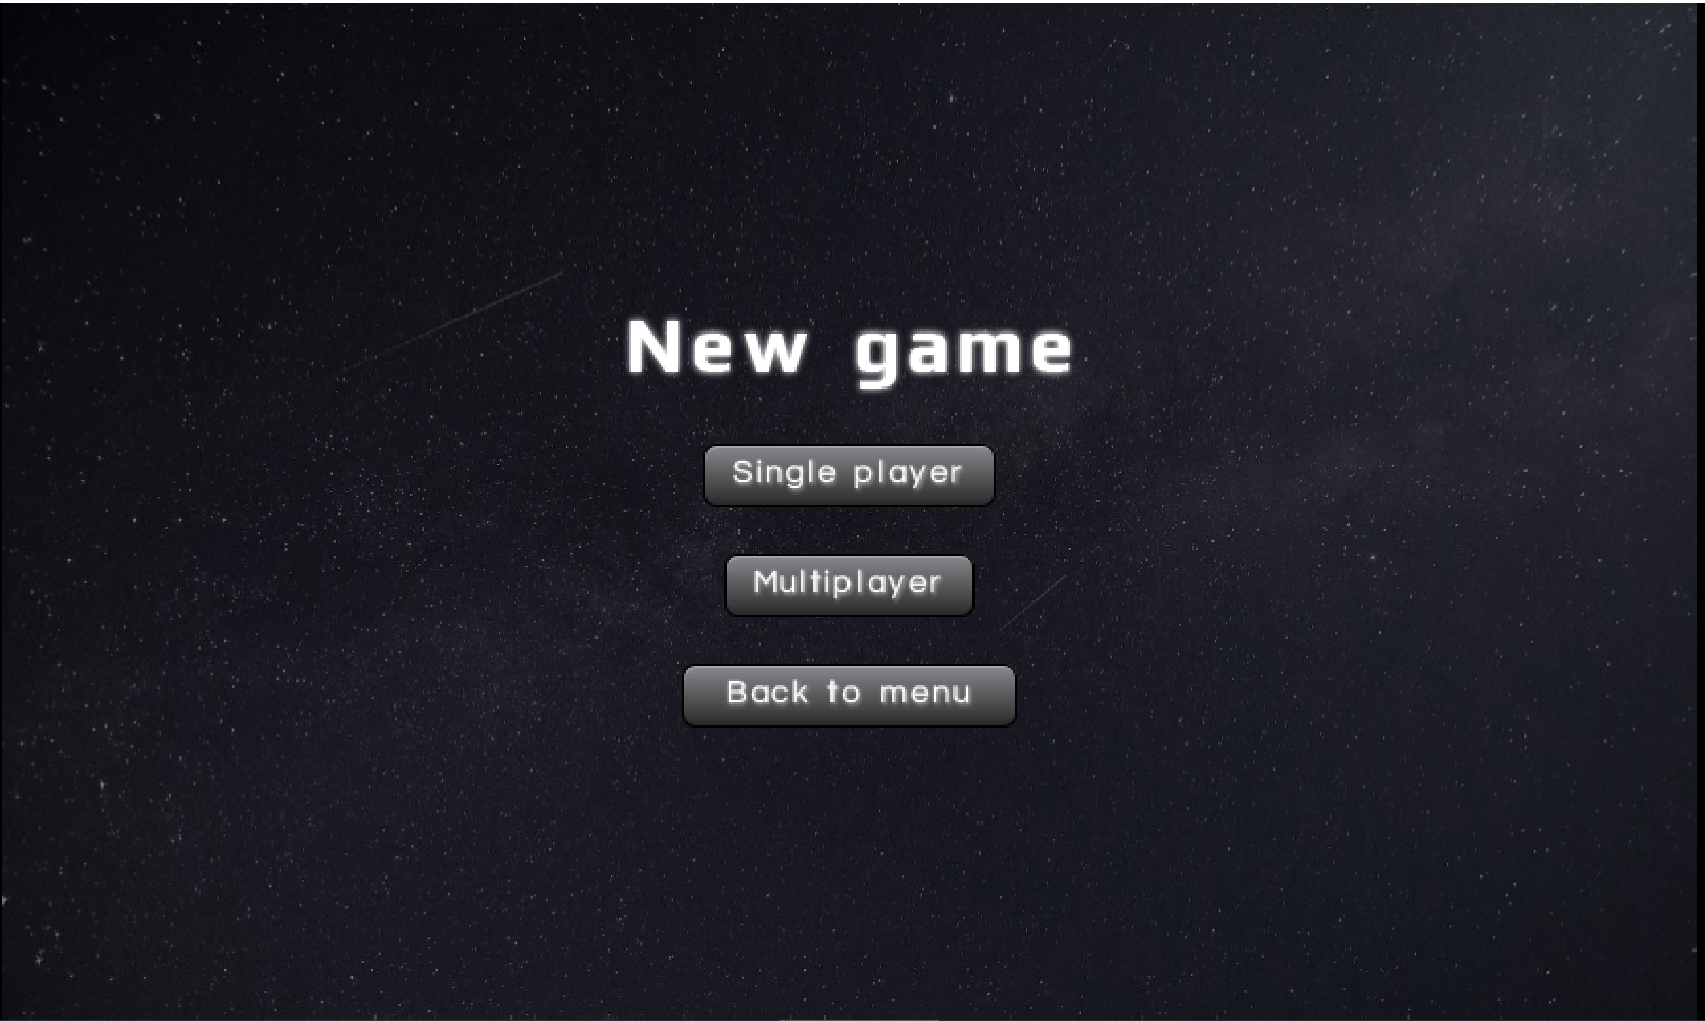
\includegraphics[width=1.00\linewidth]{pics/gamemodescreen.png}
	\caption{Spielmodus}
	%\label{fig1}
\end{figure}

\subsection{Single Player Ship Select Screen}

Hier sehen Sie den Screen, der erscheint, wenn Sie Single Player im New Game Screen gewählt haben:\\
Mittig werden die Raumschiffe angezeigt, die in dem Universum existieren, derzeit verfügt der Spieler aber nur über die Möglichkeit mit dem blauen Schiff zu spielen.\\
Über previous und next lassen sich die Raumschiffe der Zukunft anzeigen. Über den Button Show rooms unterhalb des Raumschiffs, erscheinen die Sektionen, sowie dessen Ausstattung
und Besatzung.

\begin{figure}[htp]
	\centering
	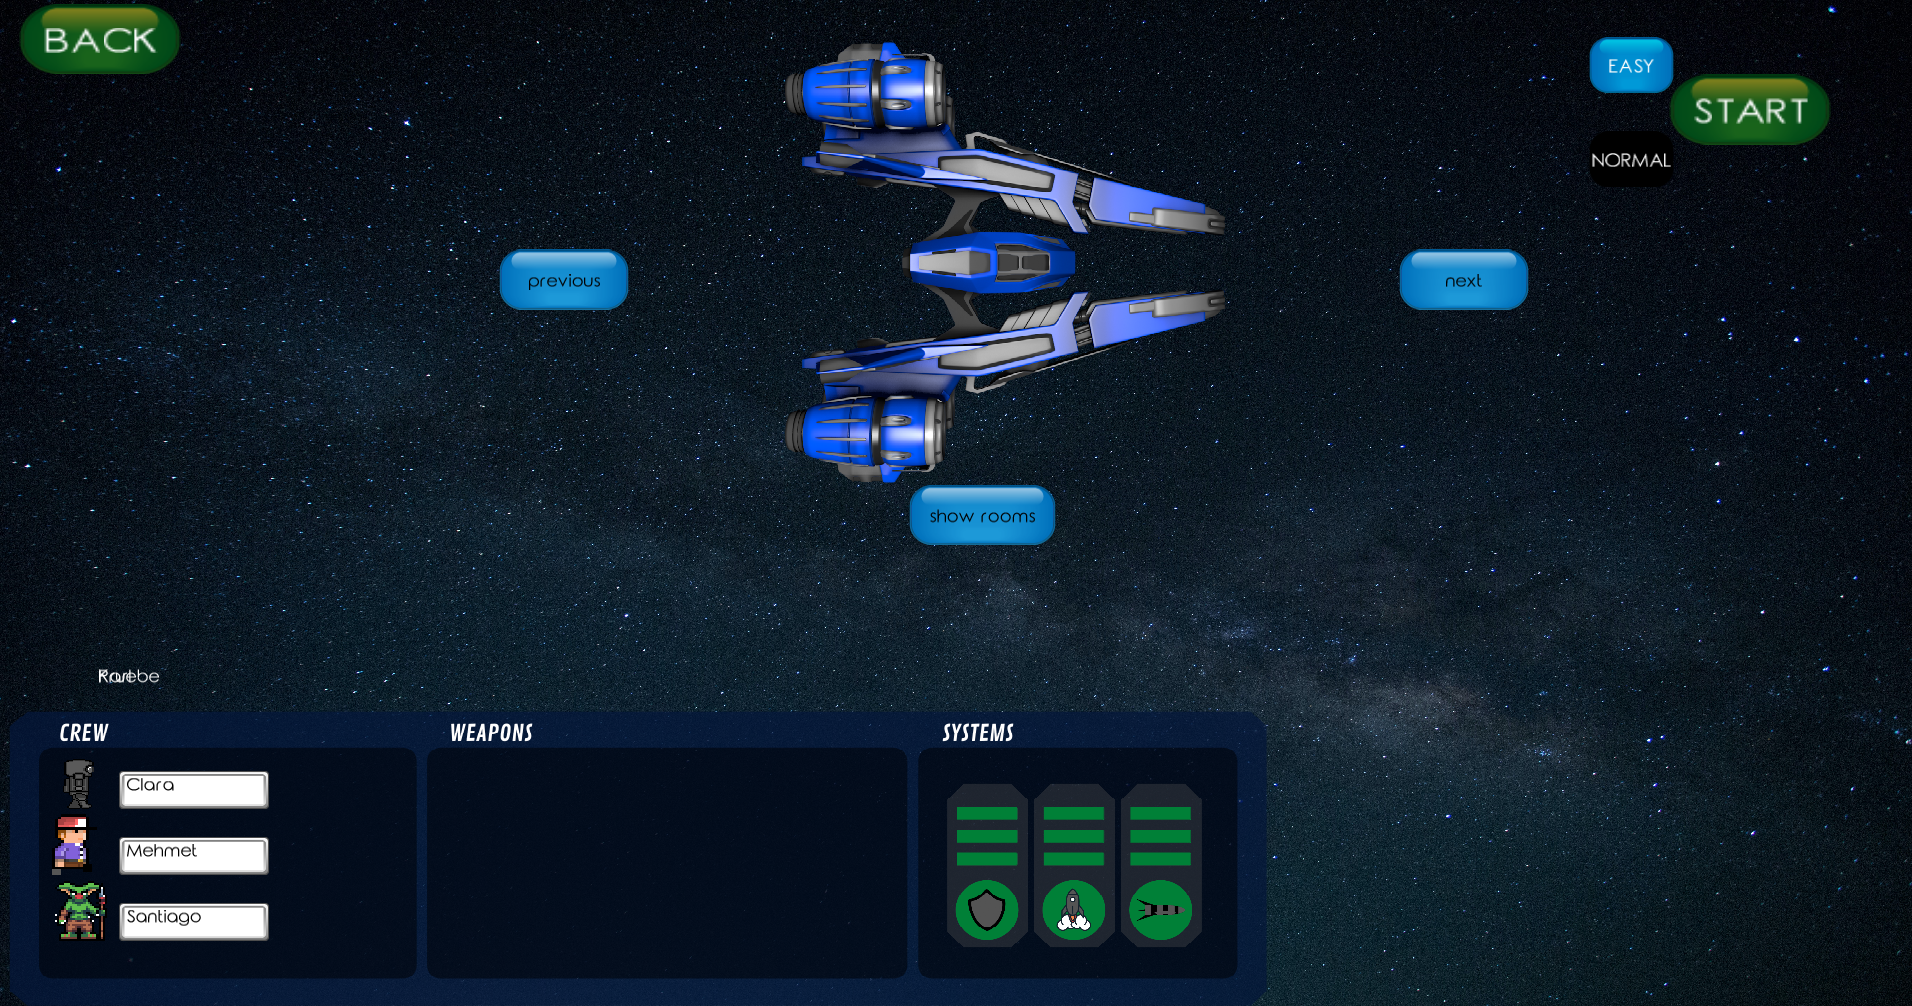
\includegraphics[width=1.00\linewidth]{pics/SinglePlayer01.png}
	\caption{Single Player}
	%\label{fig1}
\end{figure}

Die Anzeige am unteren Bildschirmrand zeigt die zugehörigen Crew Member und dessen Namen, sowie über welche Systeme das Raumschiff verfügt.\\
Links neben dem Start Button kann eine weitere Auswahl zwischen Easy und Normal getroffen werden, diese Modi entscheiden über den Schwierigkeitsgrad des Spiels.\\
Über Start beginnt das Spiel mit der Ausgewählen Spielstufe.
Der Button Back oben links in der Ecke des Fensters, leitet zurück zum New Game Screen.\\
Im Single Player Modus werden die Gegner, auf die der Spiele im laufe des Spiels trifft durch eine KI realisiert.

\newpage
%%%%%%%%%%%%%%%%%%%%%%%%%%%%%%%%%%%%%%%%%%%%%%%%%%%%%%%%%%%%%%%%%%%%%%%%
\subsection{Multiplayer Ship Select Screen}

Hier sehen Sie den Screen, der erscheint, wenn Sie  Multiplayer im New Game Screen gewählt haben:\\
Dieser Screen unterscheidet sich in sofern vom Singlaplayer Screen, dass eine zusätzliche Anzeige erscheint, der Sie entnehmen können, wie viele weitere Spieler online sind.\\
Damit weiter Spieler erscheinen, müssen diese im Login Screen die selber Netzwerkadresse angegeben haben/auf dem gleichen Server angemeldet sein und ebenfalls den Multiplayer Modus augewählt haben.\\
Außerdem entfällt die Wahl der Spielstufe, da der Gegner nun nicht mehr durch den Computer ersetzt werden muss.

\begin{figure}[htp]
	\centering
	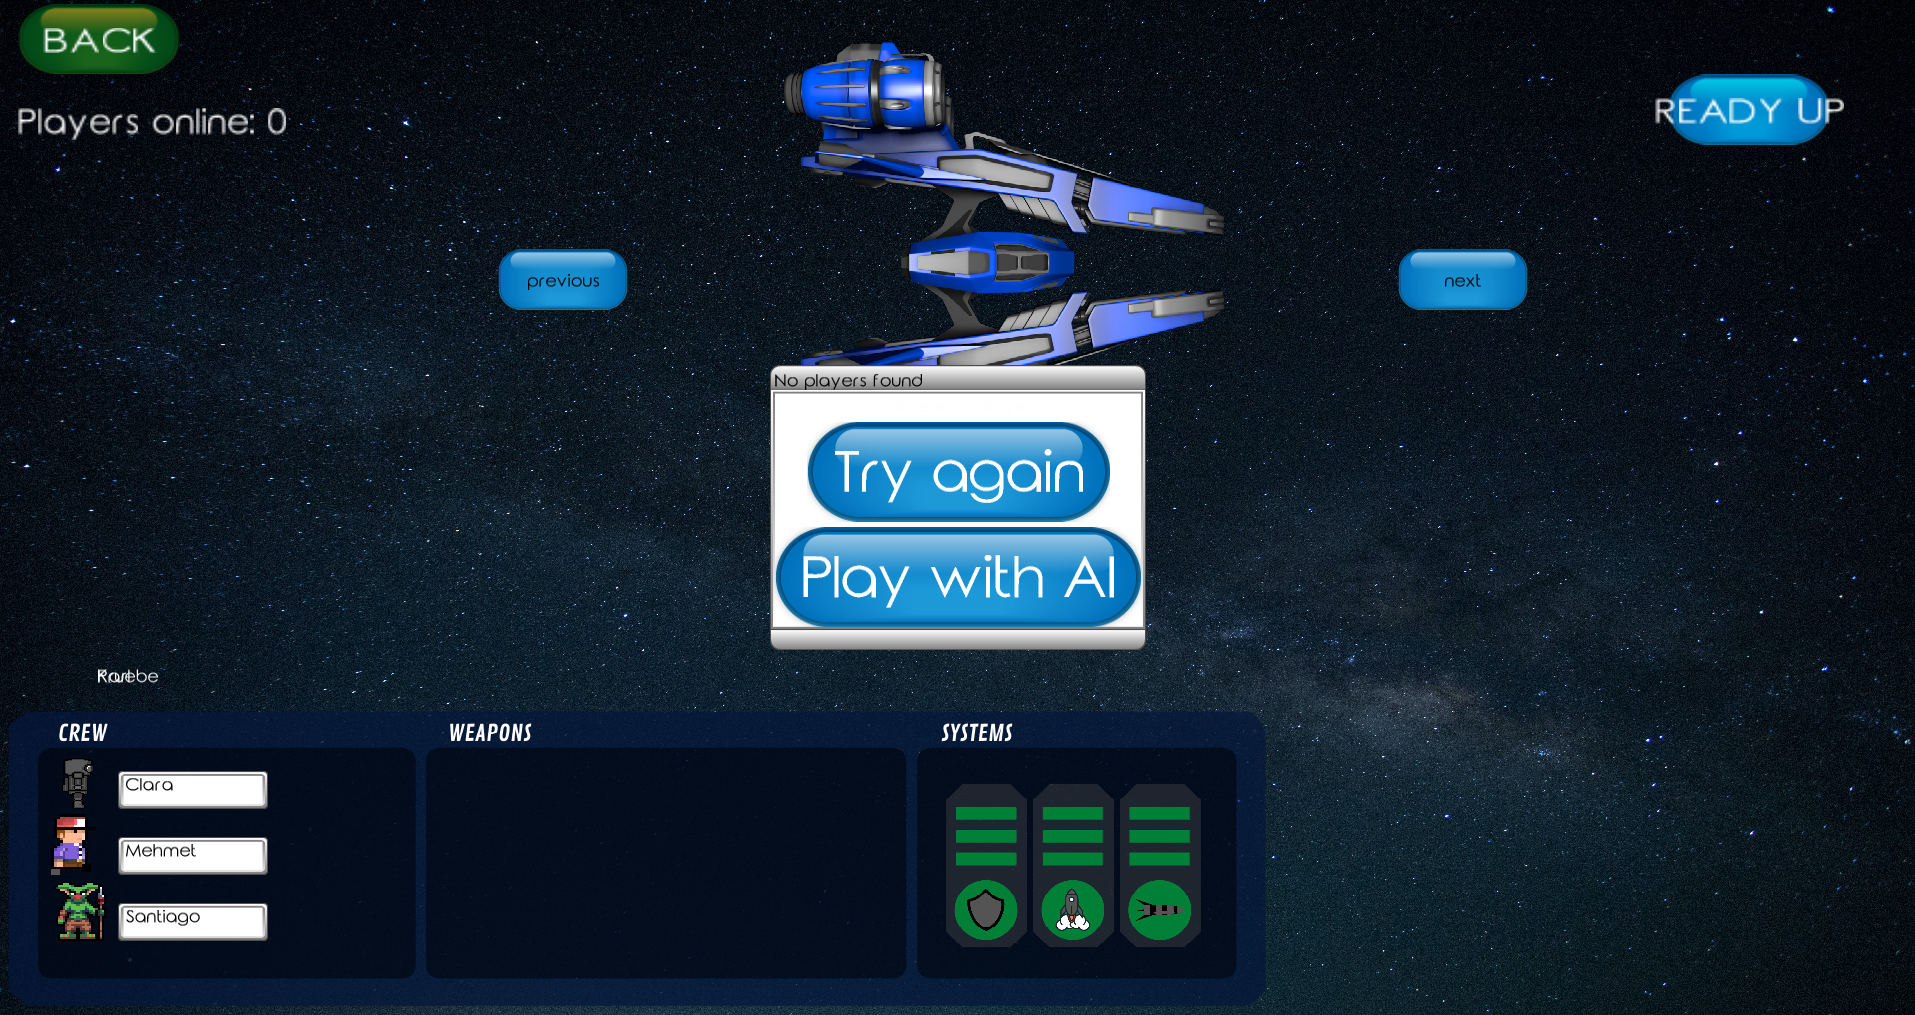
\includegraphics[width=1.00\linewidth]{pics/MultiPlayer01.png}
	\caption{Multiplayer}
	\label{fig1}
\end{figure}

Für den Fall, dass keine weiteren Spieler gefunden werden, erscheint ein Pop up Fenster das die Möglichkeiten bietet, über Try again erneut nach anderen Spielern zu suchen
oder sich über Play with AI doch zu einem Spiel im Single Player Modus umzuentscheiden.\\
 
\newpage
%%%%%%%%%%%%%%%%%%%%%%%%%%%%%%%%%%%%%%%%%%%%%%%%%%%%%%%%%%%%%%%%%%%%%%%%
\section{Univesum}

Nach klicken des Start Buttons des vorherigen Screens, gelangen Sie zur Map des Universums.\\
In diesem Beispiel sehen Sie die Map des Easy Universum. Das Raumschiff befindet sich auf dem Start Planeten unten links. Zu sehen sind vier weitere Planeten sowie eine Shoppingmall.\\
All diese Stationen können angeflogen werden.
\begin{figure}[htp]
	\centering
	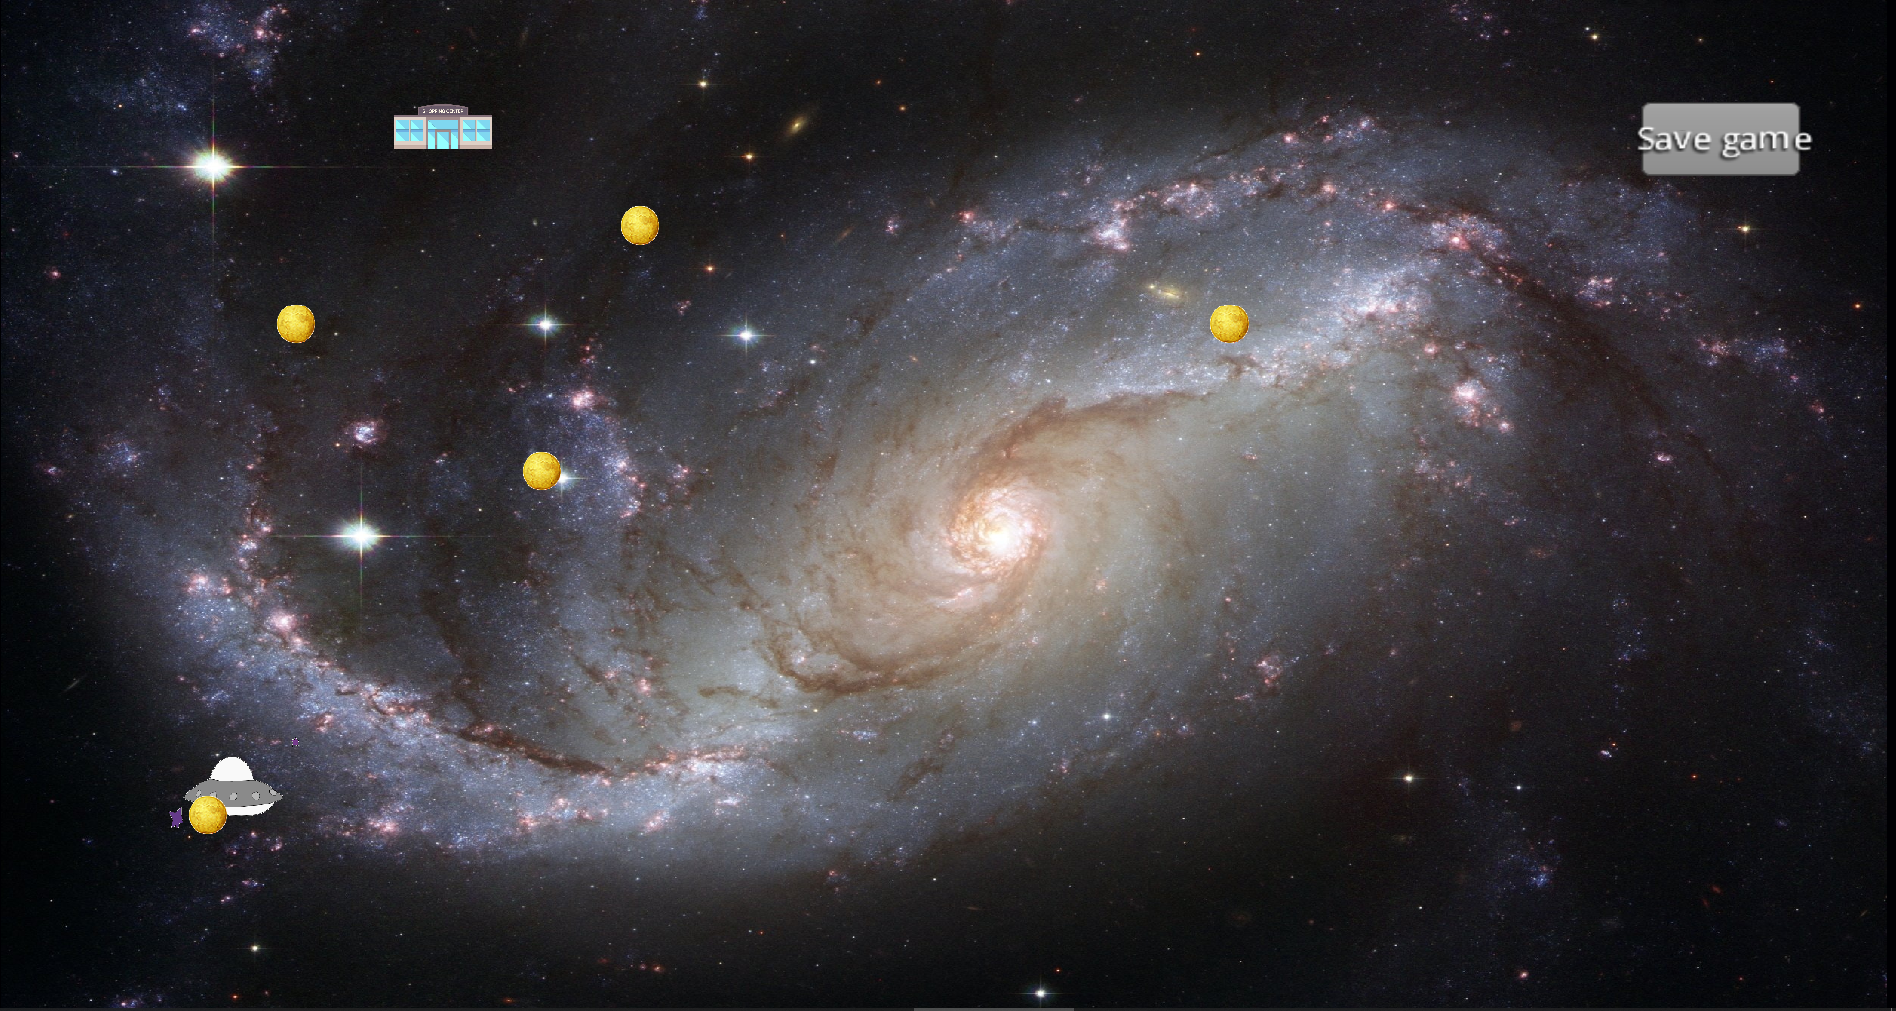
\includegraphics[width=1.00\linewidth]{pics/universeEasyP1.png}
	\caption{Map des Universums}
	\label{fig1}
\end{figure}

Wird eines der weiteren vier Planeten angeflogen (der Startplanet birgt kein Ereignis), dann erscheint ein
Pop up Fenster mit einer Information zu diesem Planeten. Die Optionen sind, per jump diesen anzufliegen und zu landen oder über back zurück zur Map zu gelangen.\\
Wird die Shopping Mall angeflogen, gelangt das Raumschiff zum Shop Screen, in dem er die Möglichkeit hat Ressourcen für sein Raumschiff einzukaufen, dazu mehr im Kapitel Shopping.\\

\begin{figure}[htp]
	\centering
	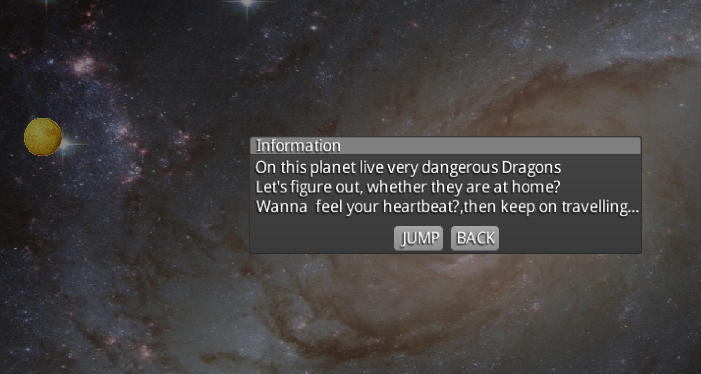
\includegraphics[width=1.00\linewidth]{pics/infoPlanet2.png} %Bild austauschen
	\caption{Info zu Planet}
	\label{fig1}
\end{figure}

Ein Planet, der bereits besucht wurde verfärbt sich dunkel:

\begin{figure}[htp]
	\centering
	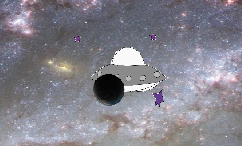
\includegraphics[width=0.30\linewidth]{pics/visitedPlanet.png}
	\caption{visited Planet}
	\label{fig1}
\end{figure}

Oben rechts im Fenster ist der Button Save game zu sehen, dieser ermöglicht das Speichern des Spiels, zu jenem Zeipunkt, wenn sich das Raumschiff wieder auf der Map befindet.

%%%%%%%%%%%%%%%%%%%%%%%%%%%%%%%%%%%%%%%%%%%%%%%%%%%%%%%%%%%%%%%%%%%%%%%%
\subsection{Einen Planeten anfliegen}
Die Planeten können in beliebiger Reihenfolge angeflogen werden, ausgenommen jener, der am weitesten östlich gelegen ist, auf diesem befindet sich der Endgegner und diesem darf sich erst dann gestellt werden, wenn alle anderen Planeten schon besucht wurden.\\
Wurde sich dann dazu entschieden per Jump einen Planeten anzufliegen, erscheint der Travelscreen.
\begin{figure}[htp]
	\centering
	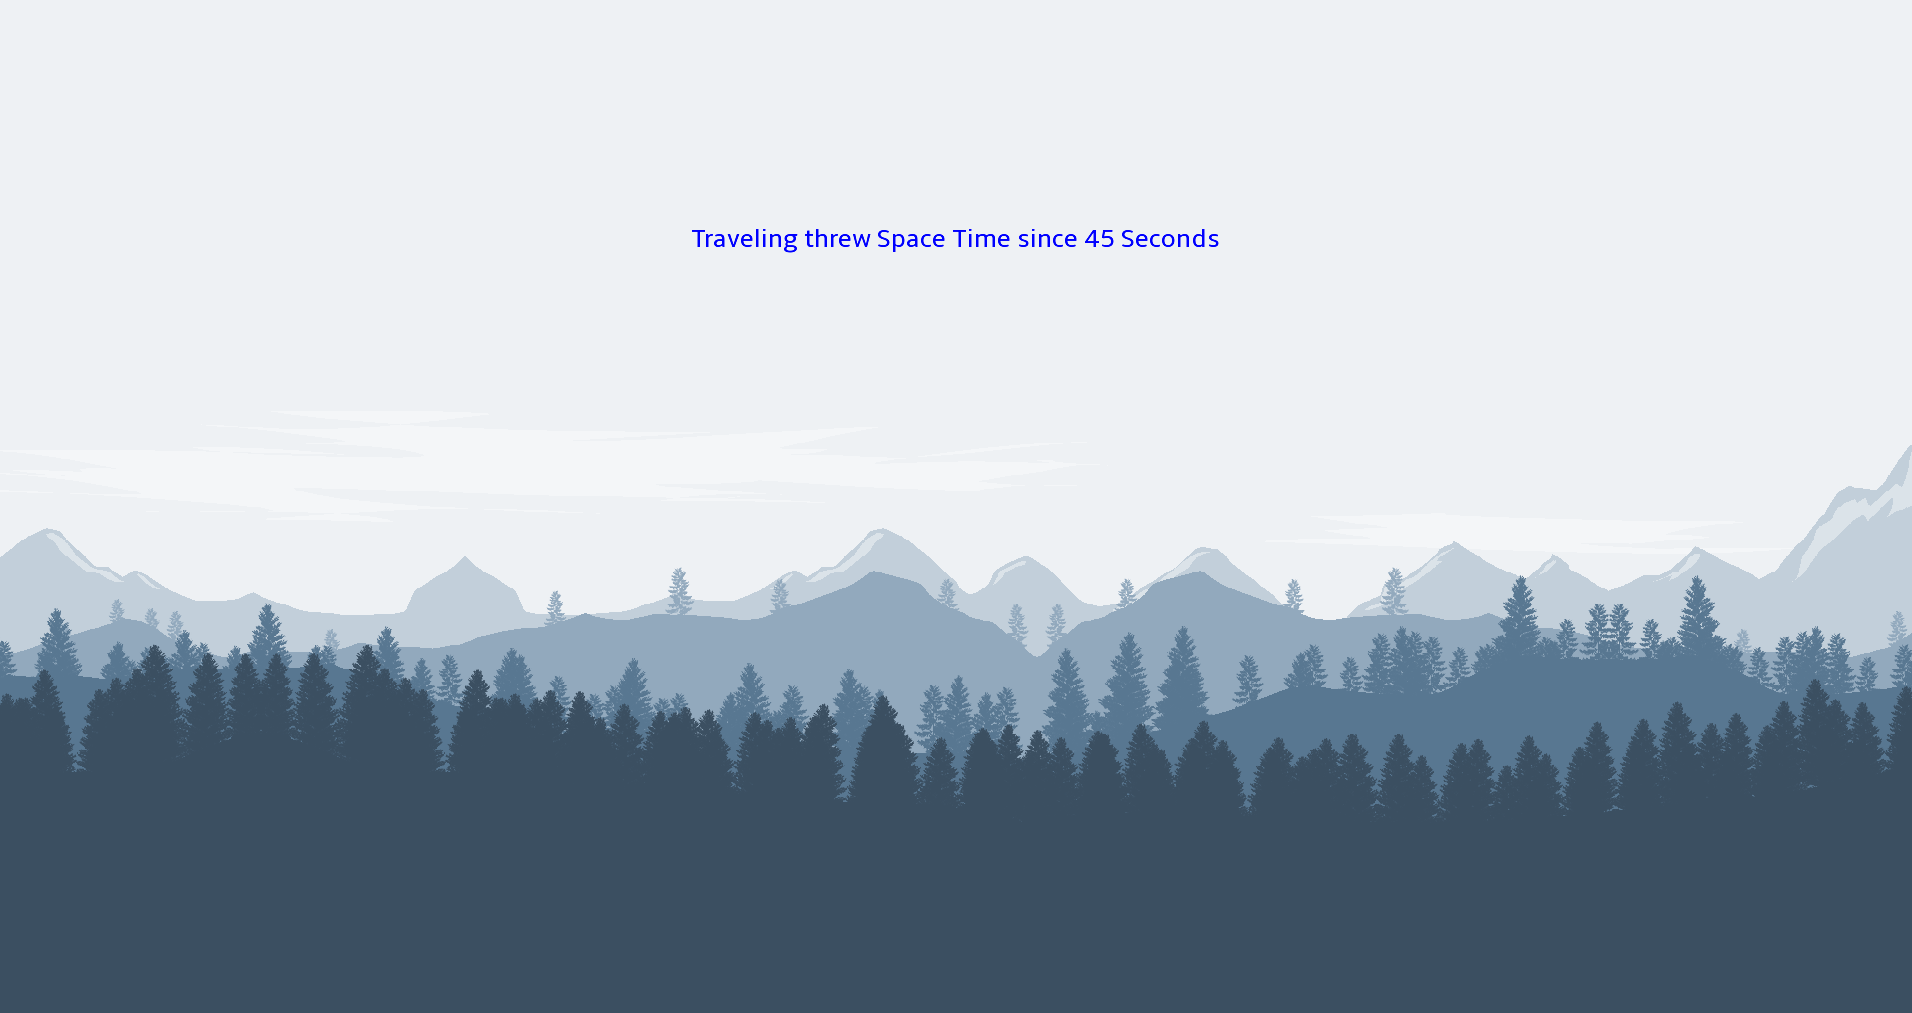
\includegraphics[width=1.00\linewidth]{pics/travelScreen.png}
	\caption{Travel Screen}
	\label{fig1}
\end{figure}
Ein Infofenster erscheint und beschreibt den Planeten, daraufhin muss sich der Spieler je nach dem, wie er die Lage einschätzt, zwischen Explore und Leave entscheiden. Leave führt zurück zur Map und Explore führt die Reise fort.\\
Nach einer kurzen Weile tritt ein zufälliges Ereignis ein, das sich positiv ode negativ auf den Spieler auswirken kann. In diesem Fall wurde das Leben/HP hochgesetzt und verändert die Anzeige unten links.\\
Je nach Ereignis, können Sie immernoch taktisch entscheiden, ob Sie fliehen, kämpfen, shoppen oder upgraden möchten.

\begin{figure}[htp]
	\centering
	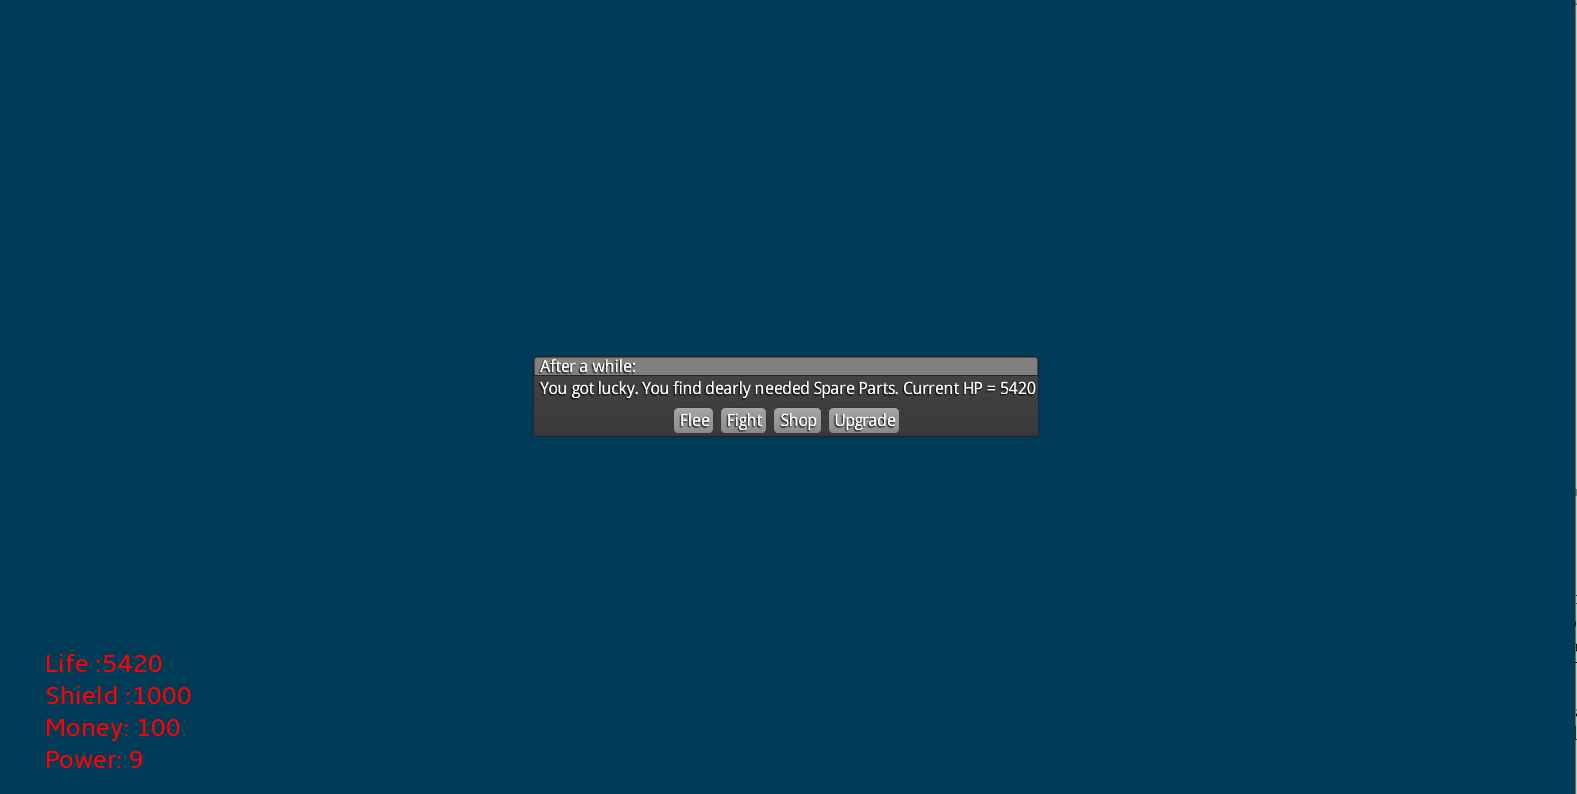
\includegraphics[width=1.00\linewidth]{pics/randomEreignis.png}
	\caption{Zufälliges Ereignis}
	\label{fig1}
\end{figure}

Über Flee gelangen Sie zurück zur Map. Über Fight treten sie unwiederruflich dem Kampf bei, über Shop wird wieder die Möglichkeit geboten zu shoppen, und über Upgrade bieten sich eine Menge Möglichkeiten, Systeme für den kommenden Kampf zu upgraden, siehe Bild.\\
Nach einem Upgrade, besteht immernoch die Möglichketi per Button wieder zurück zur Map zu gelangen.


\begin{figure}[htp]
	\centering
	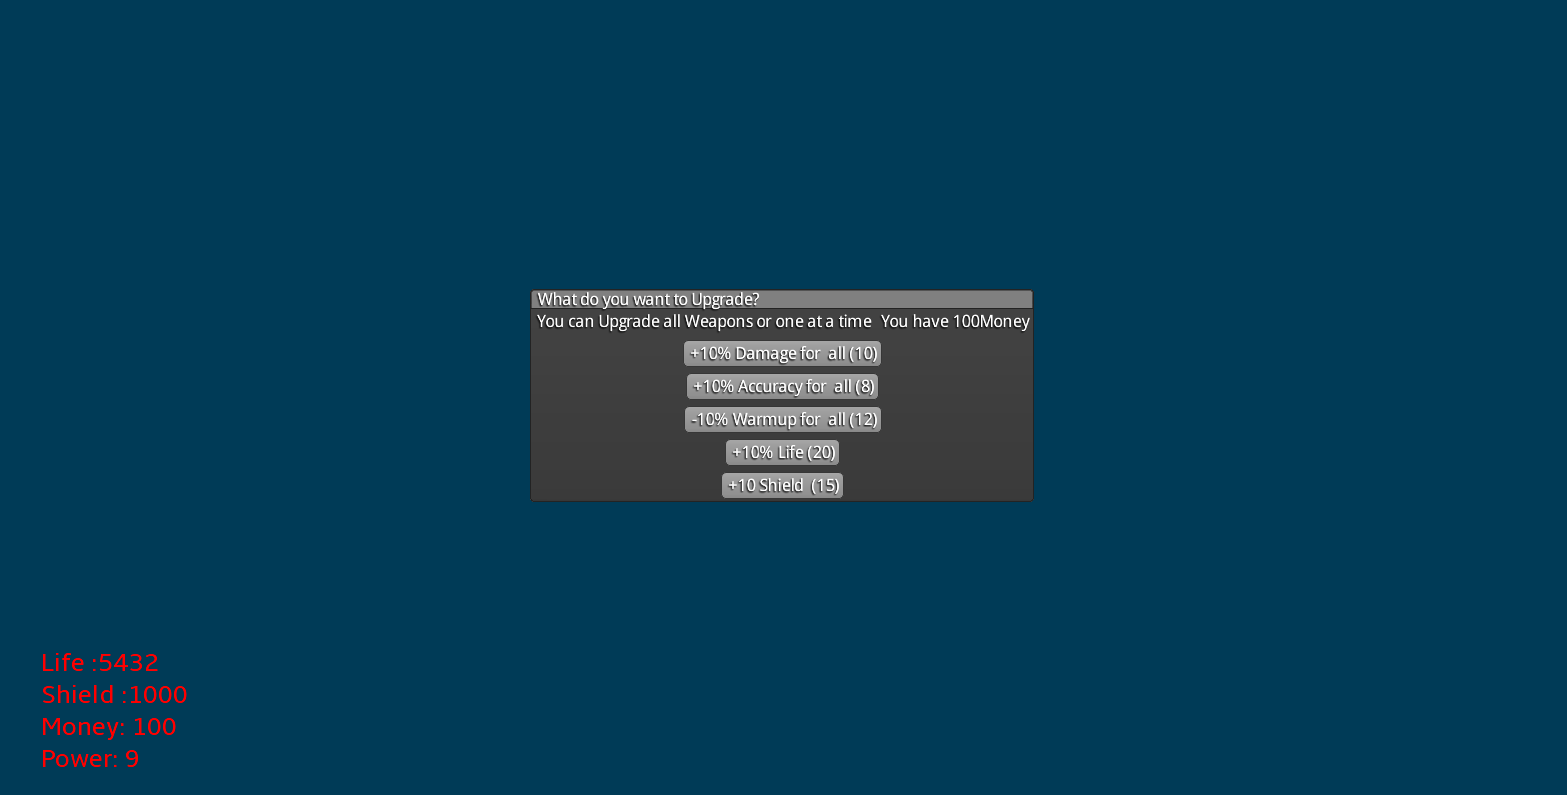
\includegraphics[width=1.00\linewidth]{pics/upgrade.png}
	\caption{Upgrade der Systeme}
	\label{fig1}
\end{figure}

%%%%%%%%%%%%%%%%%%%%%%%%%%%%%%%%%%%%%%%%%%%%%%%%%%%%%%%%%%%%%%%%%%%%%%%%
\section{Shopping}

Im Shop Screen sind drei Anzeigen zu sehen. Jene oben rechts zeigt an, wie viel Gold/Geld zur verfügung steht. Die am unteren Fensterrand beschreibt das Schiff, in diesem Fall welche Sektion für welche Systeme verantwortlich ist. Die rechte Anzeige beschreibt das Item, das darüber angezeigt wird: worum es sich handelt, Eigenschaften und dessen Kosten.\\
Über den next Button lässt sich durch das Angebot gucken, die Anzeige darunter passt sich dementsprechend an.\\
Das Angebot umfasst: Gold, Energie, Crew Member und ein Weapon Lasser. Die Kosten werden entsprechend von dem Gold abgezogen. Secure lässt sich in der vorher beschriebenen upgrade Option kaufen und nicht über den Shop.\\
Möchten Sie einen Crew Member kaufen, so muss die Checkbox der entsprechende Sektion, in die der Crew Member plaziert werden soll, ausgewählt werden, bevor der Kauf über den Buy Button bestätigt werden kann. Möchten Sie den Shop verlassen, dann klicken Sie auf den Back to Map Button in der oberen rechten Ecke. 

\begin{figure}[htp]
	\centering
	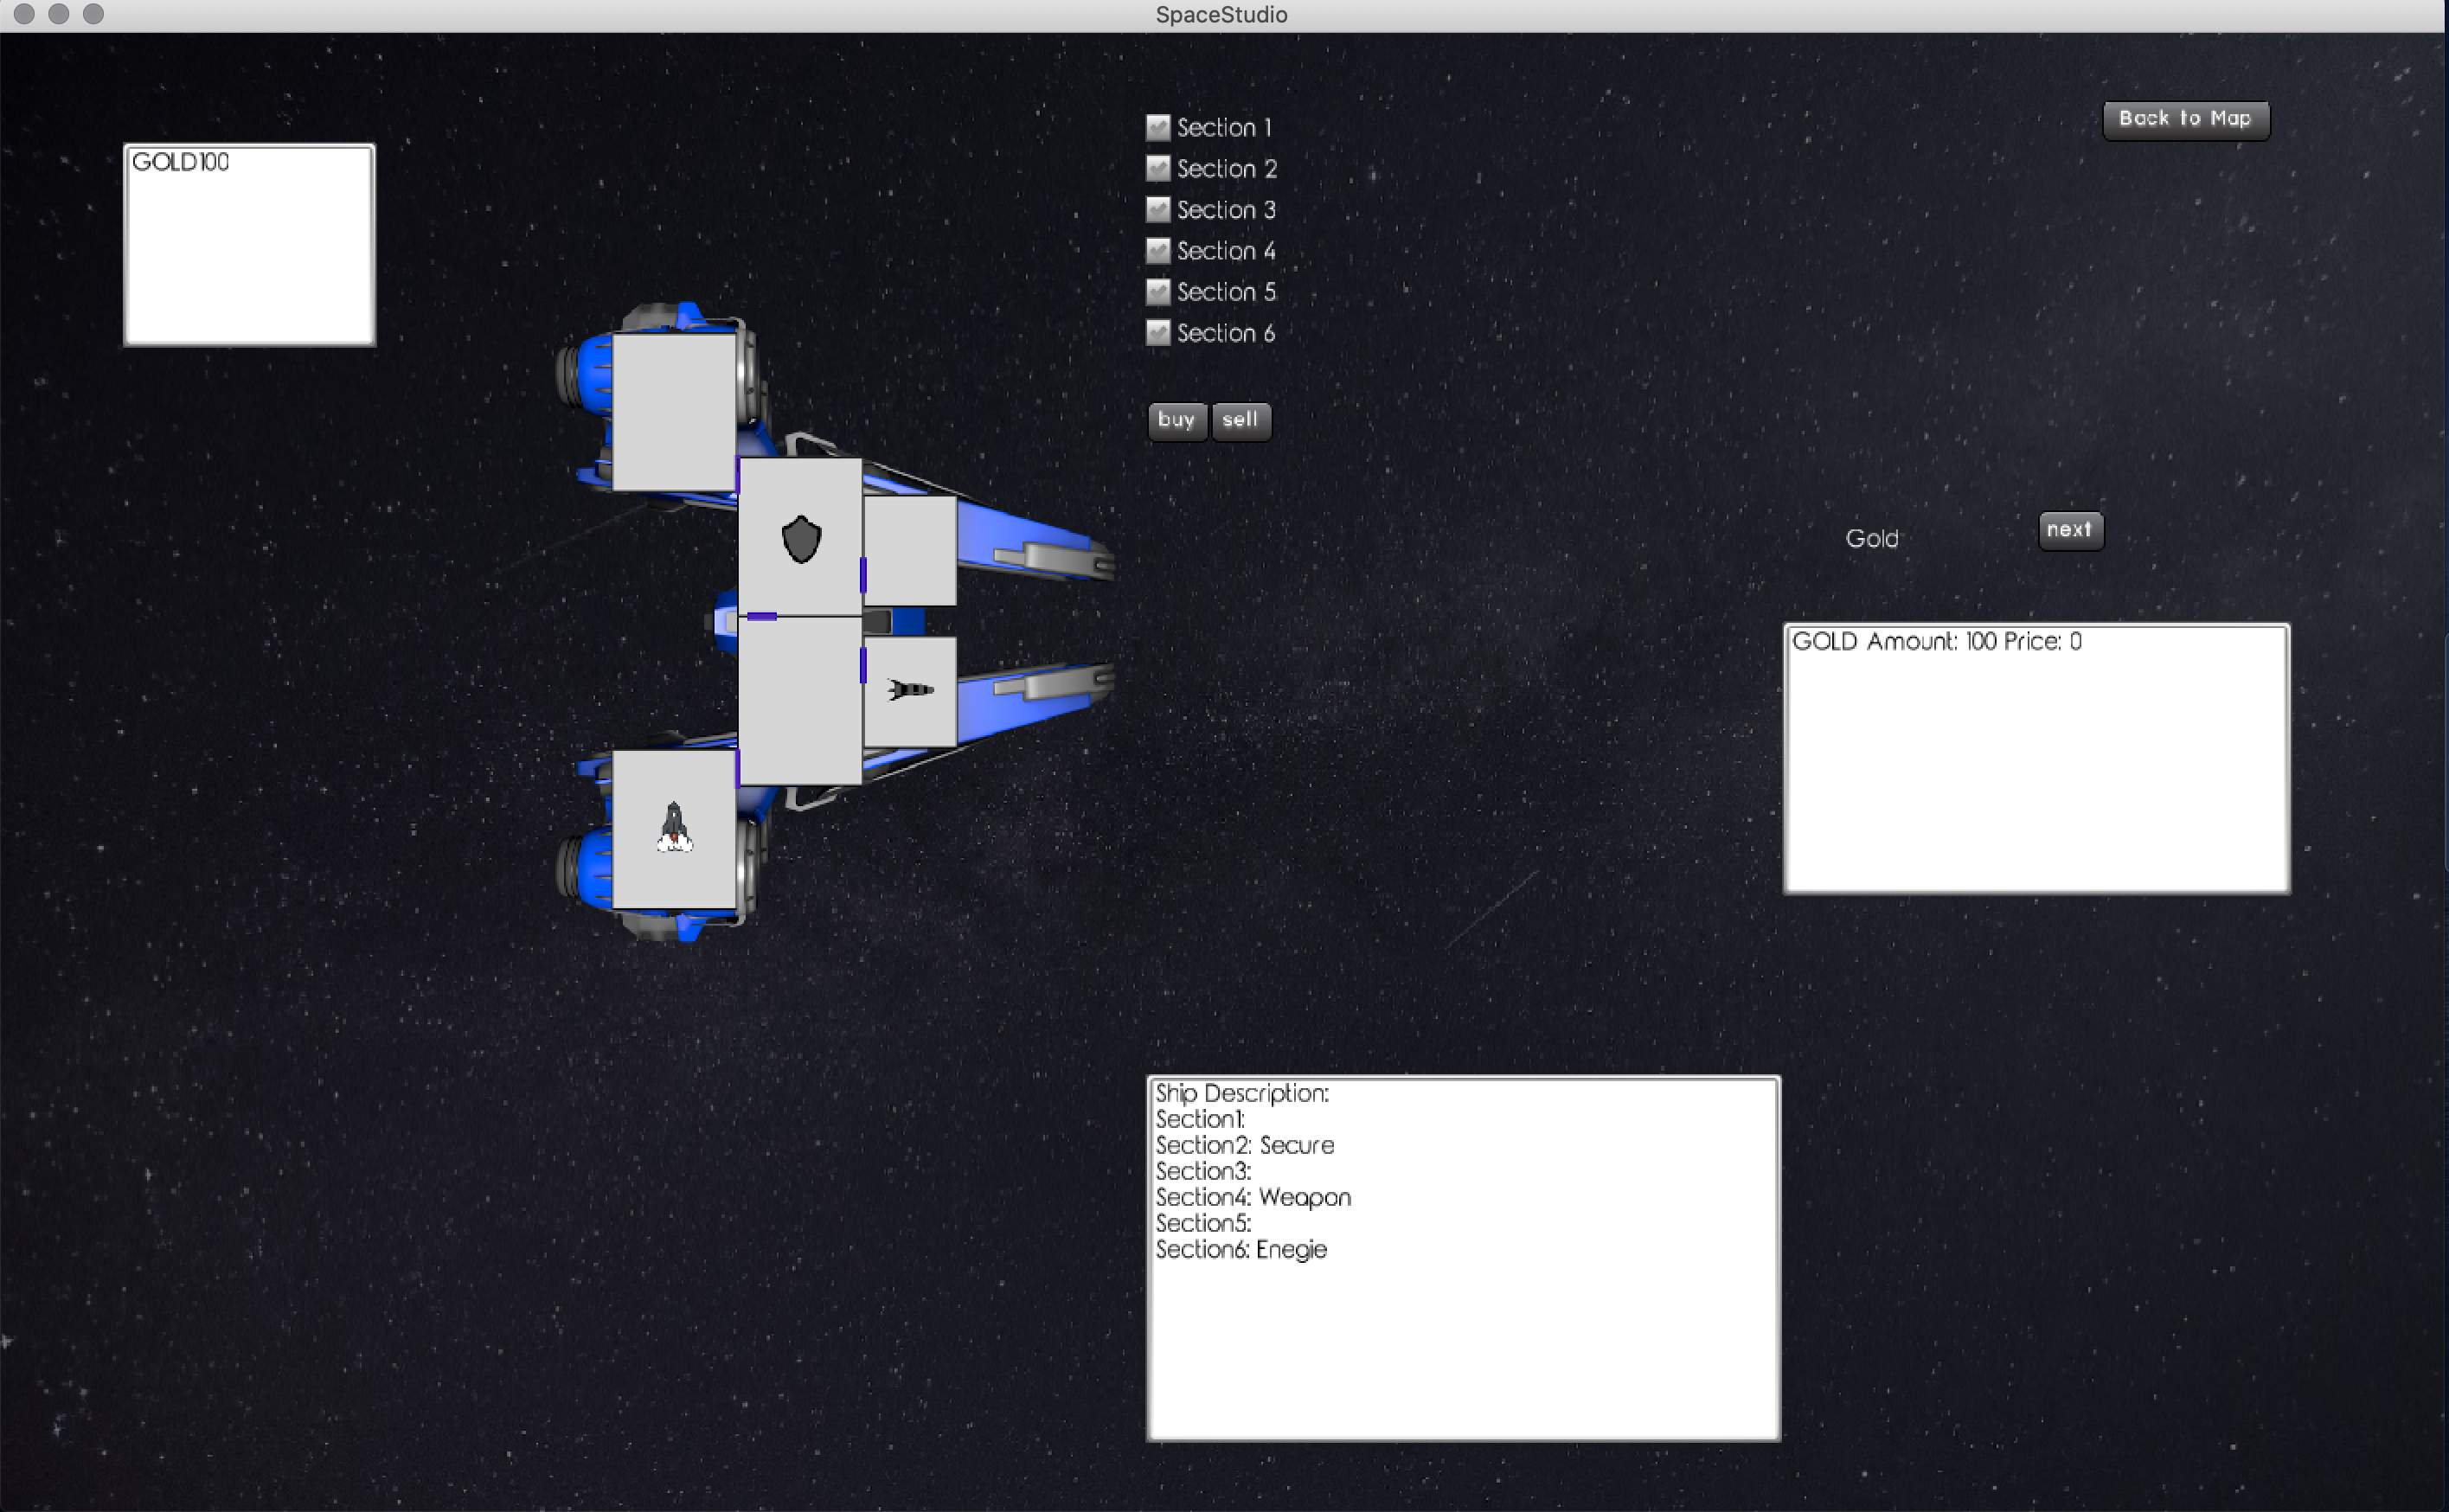
\includegraphics[width=1.00\linewidth]{pics/shopScreen.png} %Bild muss noch angepasst werden ohne Sell button
	\caption{Shop}
	\label{fig1}
\end{figure}

%%%%%%%%%%%%%%%%%%%%%%%%%%%%%%%%%%%%%%%%%%%%%%%%%%%%%%%%%%%%%%%%%%%%%%%%
\section{Der Kampf}

\subsection{Beschreibung der Oberfläche}
Im Kampf stehen sich das Raumschiff des Spielers und das des Gegners gegenüber.
Zu Beginn sind die Raumschiffe jeweils von ihrem Schutzschild umgeben.
Die Schrift auf der linken Seite des Fensters beschreibt die Waffen des eigenen Raumschiffs.
In diesem Fall verfügt das Raumschiff des Spielers über die Waffen Rocket Left und Lasser Right.
Diese wiederum haben die Attribute Damage, Bullets und Warmup. Damage gibt an, wie viel Schaden die Waffe dem Gegner bei einem Treffer zufügt. Die Anzahl der Bullets sind
die Anzahl der Schüsse einer Waffe und Warmup gibt die Dauer in Runden an, bis die Waffe wieder einsatzbereit ist.\\

Unten links ist die Energie und dessen Verteilung zu sehen. In dem weißen Balken von links nach rechts: der Betrag des Schutzschildes, das Leben des Gegners (Hp), Secure, Drive und Weapon.
Die grünen Balken stellen die Energie dar, die verteilt werden kann.\\

Die eigenen Sektionen und dessen Eigenschaften sind in roter Schrift unterhalb des gegnerischen Raumschiffs beschrieben: ist die Sektion benutzbar, wie viel Oxygen ist in der Sektion verfügbar, welche Rolle hat die Sektion, dh. für welches System ist sie verantwortlich, ob Health, Weapon oder Engine und welcher Crew Member ist anwesend.\\

In dem gegnerischen Raumschiff sind drei weiße Symbole zu sehen. Diese repräsentieren die Systeme, die angegriffen werden müssen. In diesem Fall hat das gegnerische Raumschiff
ein Cockpit, ein Drive System und ein Weapon System.\\ 

Der Button, welche unten mittig des Fensters zu finden ist, zeigt entweder Waiting oder Playing an,
je nach dem, ob der Spieler oder der Gegner am Zug ist.

\begin{figure}[htp]
	\centering
	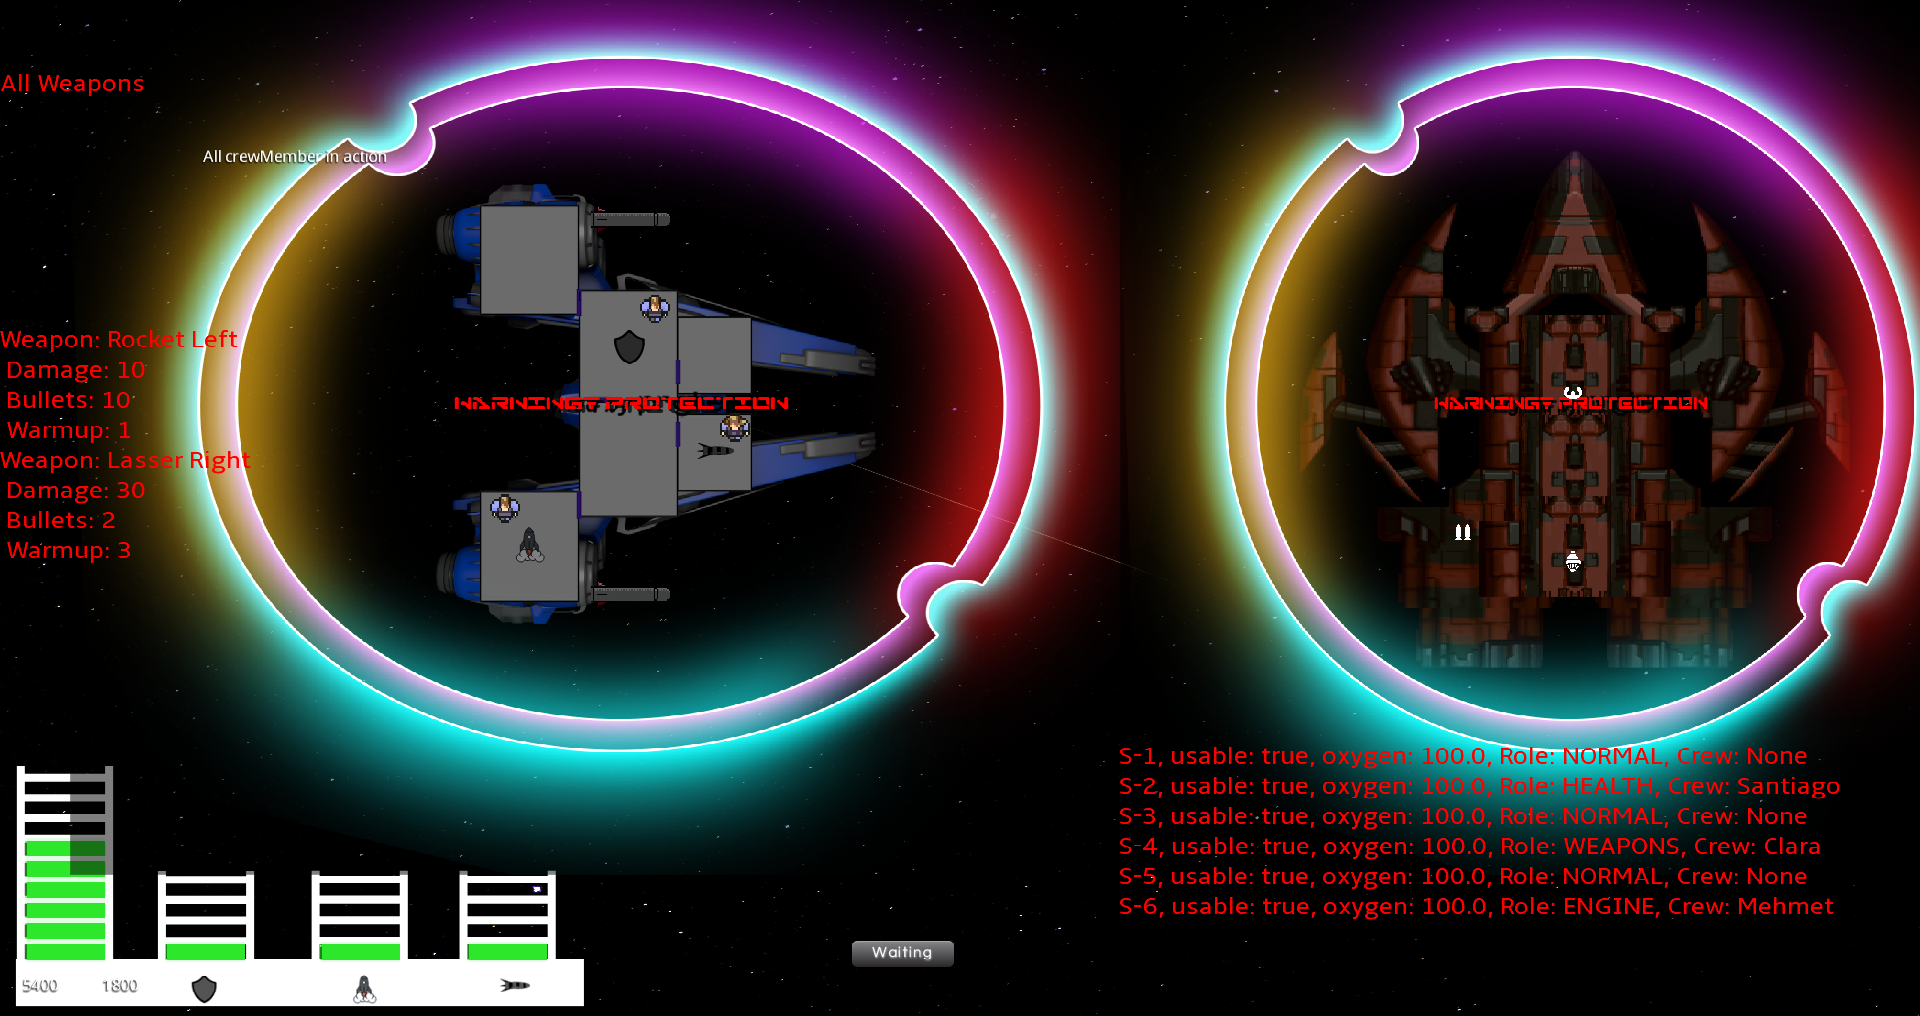
\includegraphics[width=1.00\linewidth]{pics/combatScreenRot01.png}
	\caption{der Kampf}
	\label{fig1}
\end{figure}

\subsection{Spielverlauf}

Um den Kampf zu starten, klicken Sie bitte auf den waiting Button und anschließend erneut
auf Playing.\\

Wie schon erwähnt, sind beide Raumschiffe von ihren Schutzschildern umgeben, diese halten einige 
Schüsse ab, bis sie verschwinden. Erst dann wenn dieser Schutz aufgehoben ist, sind die Raumschiffe und somit auch dessen Sektionen und Systeme verletzlich.\\

Wählen Sie ein System des Geners aus, z.B das Cockpit, um auf dieses zu schießen. Die Auwahl kann nach jedem Schuss verändert werden. Haben Sie diesen
Schritt vergessen, erscheint ein Pop up: Please select a target. Then you can shoot.\\

Nun können Sie über die Leertaste die Schüsse der Waffe abfeuern. 
Bullets zeigt dynamisch die verbleibenden Schüsse an. Die Waffe ist nur dann einsatzbereit, wenn Warmup auf 0 ist. Warmup zählt, pro Spielzug, die des Gegners zählen mit, runter. Sind keine Schüsse mehr übrig, ist die Runde beendet.
In einer Runde wird automatisch nur die Waffe verwendet, dessen Warup auf 0 ist.
Trifft der Gegner eine Sektoin des Spielers, kann einem Pop Up entnimmen werden, welcher Sektion ein Schaden zugefügt wurde.\\

Je Runde wird dem Spieler neue Energie zugewiesen, die er per klick auf den jeweiligen Balken auf die Systeme Secure, Weapon und Drive
verteilen kann.\\

Hat das Weapon System keine Energie, kann nicht geschossen werden, ein Pop Up mit dem Hinweis:
Please charge energy to the weaponsystem, erscheint.
Durch das verteilen der Energie auf das Sercure System, kann es länger aufrecht erhalten werden. Ist es jedoch einmal zerstört worden und verschwunden, kann es durch weitere Energie nicht wieder hergestellt werden. --was wenn drive keine energie hat?--\\

Der Spieler hat nicht nur die Möglichkeit zu schießen, sonder auch die Crew Member zu bewegen.
Die Anwesenheit eines Crew Members wirkt sich auf die Systeme in der jeweiligen Sektion aus.
Ist usable: false für eine Sektion, dann wird sie automatisch durch den anwesenden Crew Member repariert.\\
 Ein Crew Member lässt sich ganz einfach per Drag and Drop von Sektion zu Sektion bewegen.
Hat sich dieser bewegt, erscheint eine Sanduhr neben seinem Kopf, welche signalisiert, dass der Crew Member noch Zeit für den Sektionswechsel benötigt. Die Sanduhr verschwindet, sobald diese abgelaufen ist
 und erst dann kann sich dessen Anwesenheit wieder auf die Systeme der entsprechenden Sektion auswirken. Ist das Oxygen einer Sektion unter 30\%, dann sterben die Crew Member, die sich in dieser aufgehalten haben. Ein Pop Up mit dem Hinweis: You have lost a Crew Member, erscheint. Crew wird in der Anzeige auf None gesetzt.
Der Rest passiert Backend, das Image und der Geist bleiben erhalten, die Funktionalität jedoch ist aufgehoben. --reparatur rollenabhängig?--\\

Wann und ob ein System des Geners erfolgreich zerstört wurde, ist nicht ersichtlich.
Dies bezüglich, muss die Crew auf ihre Erfahrung zurückgreifen und den Sachverhalt intuitiv abschätzen.\\

Der Kampf ist gewonnen, wenn alle Systeme des Gegners erfolgreich zerstört wurden und dessen Hp somit auf weniger als 1 gesunken ist (kann der Anzeige im weißen Balken entnommen werden).
Wurde das Spiel gewonnen, erscheint ein Pop Up mit dem Hinweis: Congratulations!! You won this fight. But 
the game is not over yet. Das gesamte Spiel ist nämlich erst dann zu Ende, wenn alle Planeten besucht wurden und schließlich der letzte Planet angeflogen werden kann, auf dem der Endgegner ungedultig auf den Spieler wartet.\\

Der Kampf ist verloren, wenn keine Sektion mehr usable ist. Das ist der Fall, wenn entweder kein Oxygen mehr verfügbar ist, die darin enthaltene System zerstört wurden, oder aber das Hp des Spielers unter 1 ist.
-- eigene hp anzeige? --
Dem Spieler erscheint ein Hinweis, dass er verloren hat und wird umgehend zurück zum New Game Screen
zurück geleitet.\\


%%%%%%%%%%%%%%%%%%%%%%%%%%%%%%%%%%%%%%%%%%%%%%%%%%%%%%%%%%%%%%%%%%%%%%%%
\subsection{Spielverlauf beim Multiplayer Modus}
Beschreibung der Kamfscreen.

%%%%%%%%%%%%%%%%%%%%%%%%%%%%%%%%%%%%%%%%%%%%%%%%%%%%%%%%%%%%%%%%%%%%%%%%
\subsection{Spielstufen}

Das Universum Easy ist im Kapitel Universum abgebildet. In dieser Abbildung ist das Universum Normal zusehen. Die Map untercheidet sich optisch nur in der Anzahl der Planeten.
Der unterschied der Spielstufen besteht darin, dass im Normal Modus mehr Gegner besiegt werden müssen, 
um das gesammte Spiel zu gewinnen, als im Easy Modus.

\begin{figure}[htp]
	\centering
	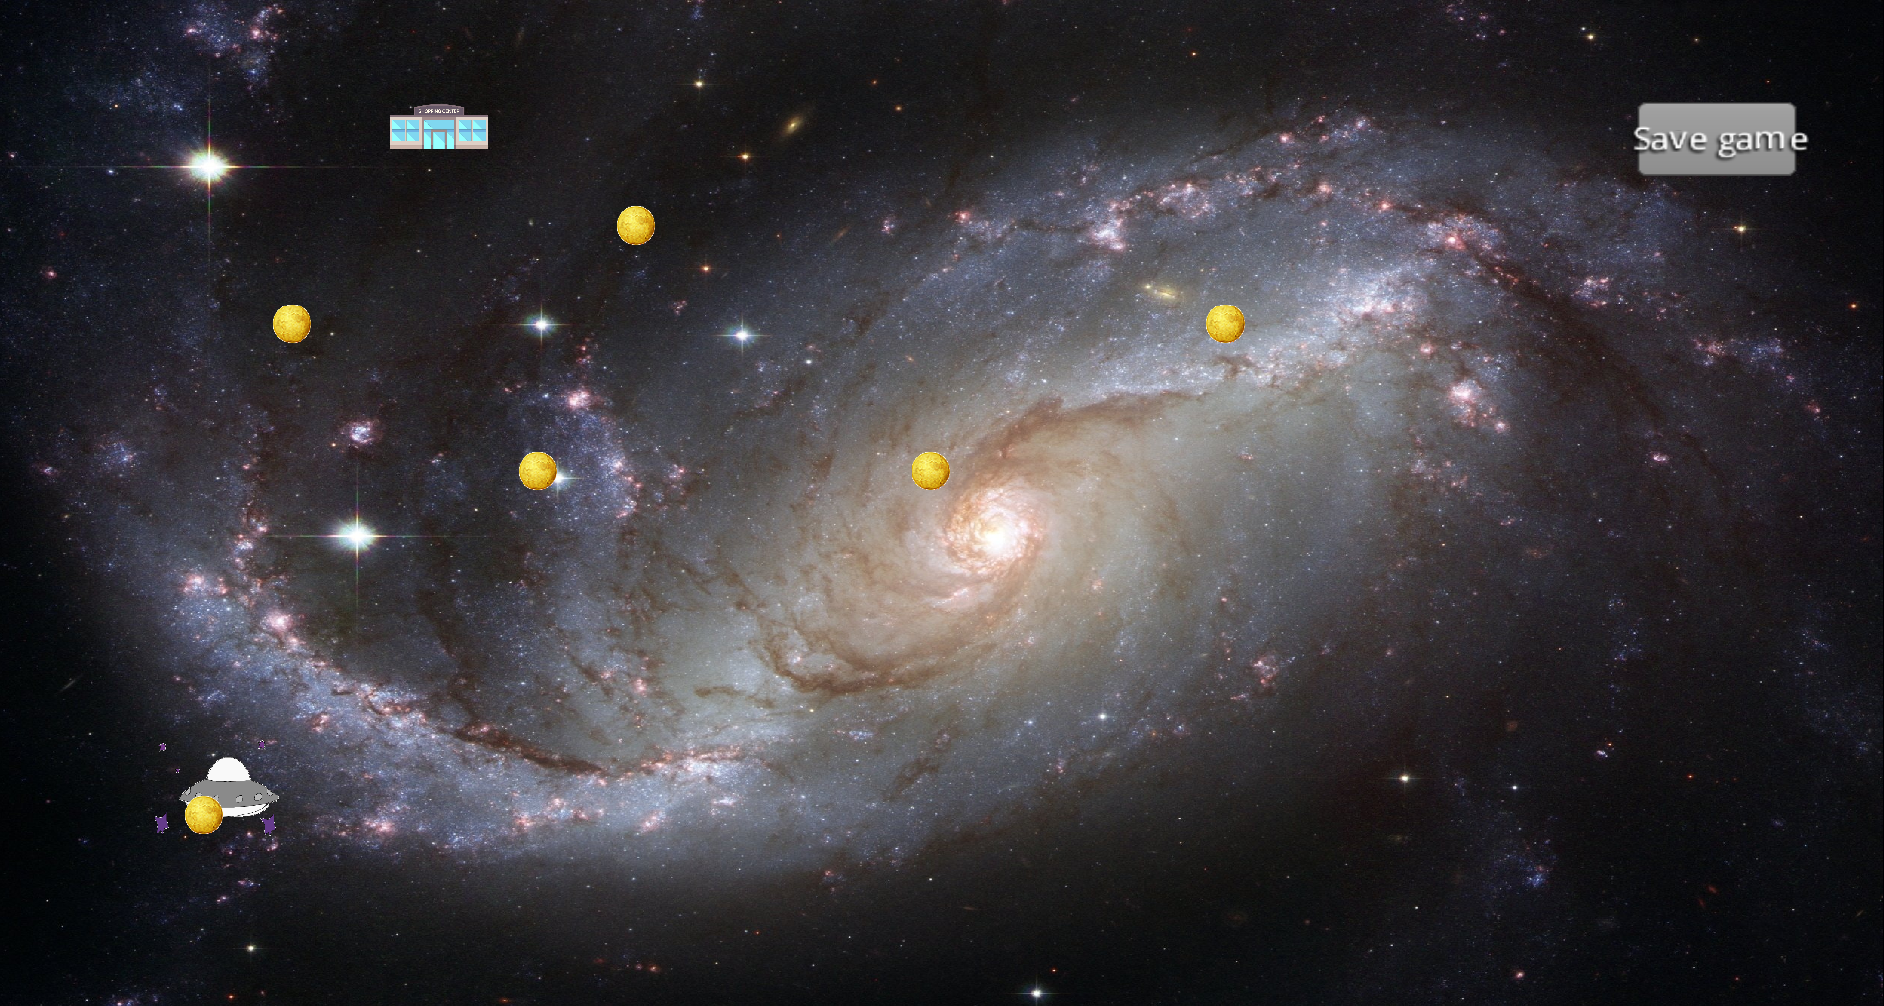
\includegraphics[width=1.00\linewidth]{pics/universumNormal.png}
	\caption{Universum Normal}
	\label{fig1}
\end{figure}

%%%%%%%%%%%%%%%%%%%%%%%%%%%%%%%%%%%%%%%%%%%%%%%%%%%%%%%%%%%%%%%%%%%%%%%%


\section{Save Game \& Continue}

Das Spiel lässt sich nach jeder Runde speichern. Eine Runde bedeutet der Besuch eines Planeten.
Ist der Spieler also zurück zur Map gelangt, kann der Save Game Button benutz werden.
Bei einer erneuten Anmeldung über die Login Felder im Login- und Registrierungs Screen mit dem selben
Benutzernamen und Passwort, hat der Spieler im New Game Screen zusätzlich die Möglichkeit, den Continue
Button zu benutzen. In diesem Fall muss das Spiel nicht neu begonnen werden, der Besuch jedes einzelnen Planeten und der Zustand des Raumschiffes mit all seinen Attributen wurde gespeichert.

\section{Anhang}
\subsection{Autoren}

\end{document}

%%% Local Variables: 
%%% mode: latex
%%% mode: reftex
%%% mode: flyspell
%%% ispell-local-dictionary: "de_DE"
%%% TeX-master: t
%%% End: 
